% Sample tex file for usage of iidef.sty
% Homework template for Inference and Information
% UPDATE: October 12, 2017 by Xiangxiang
% UPDATE: 22/03/2018 by zhaofeng-shu33
\documentclass[a4paper]{article}
\usepackage[T1]{fontenc}
\usepackage{amsmath, amssymb, amsthm}
% amsmath: equation*, amssymb: mathbb, amsthm: proof
\usepackage{moreenum}
\usepackage{mathtools}
\usepackage{url}
\usepackage{graphicx}
\usepackage{subcaption}
\usepackage{booktabs} % toprule
\usepackage[mathcal]{eucal}
\usepackage{dsfont}

\usepackage{setspace}  
\setstretch{1.6}








\theoremstyle{definition}
\newtheorem{definition}{Definition}[section]
\newtheorem{example}[definition]{Example}
\newtheorem{exercise}[definition]{Exercise}
\newtheorem{remark}[definition]{Remark}
\newtheorem{observation}[definition]{Observation}
\newtheorem{assumption}[definition]{Assumption}
\newtheorem{convention}[definition]{Convention}
\newtheorem{priniple}[definition]{Principle}
\newtheorem{notation}[definition]{Notation}
\newtheorem*{axiom}{Axiom}
\newtheorem{coa}[definition]{Theorem}
\newtheorem{srem}[definition]{$\star$ Remark}
\newtheorem{seg}[definition]{$\star$ Example}
\newtheorem{sexe}[definition]{$\star$ Exercise}
\newtheorem{sdf}[definition]{$\star$ Definition}
\newtheorem{question}{Question}




\newtheorem{problem}{Problem}
%\renewcommand*{\theprob}{{\color{red}\arabic{section}.\arabic{prob}}}
\newtheorem{rprob}[problem]{\color{red} Problem}
%\renewcommand*{\thesprob}{{\color{red}\arabic{section}.\arabic{sprob}}}
% \newtheorem{ssprob}[prob]{$\star\star$ Problem}



\theoremstyle{plain}
\newtheorem{theorem}[definition]{Theorem}
\newtheorem{Conclusion}[definition]{Conclusion}
\newtheorem{thd}[definition]{Theorem-Definition}
\newtheorem{proposition}[definition]{Proposition}
\newtheorem{corollary}[definition]{Corollary}
\newtheorem{lemma}[definition]{Lemma}
\newtheorem{sthm}[definition]{$\star$ Theorem}
\newtheorem{slm}[definition]{$\star$ Lemma}
\newtheorem{claim}[definition]{Claim}
\newtheorem{spp}[definition]{$\star$ Proposition}
\newtheorem{scorollary}[definition]{$\star$ Corollary}


\newtheorem{condition}{Condition}
\newtheorem{Mthm}{Main Theorem}
\renewcommand{\thecondition}{\Alph{condition}} % "letter-numbered" theorems
\renewcommand{\theMthm}{\Alph{Mthm}} % "letter-numbered" theorems


%\substack   multiple lines under sum
%\underset{b}{a}   b is under a


% Remind: \overline{L_0}



\usepackage{calligra}
\DeclareMathOperator{\shom}{\mathscr{H}\text{\kern -3pt {\calligra\large om}}\,}
\DeclareMathOperator{\sext}{\mathscr{E}\text{\kern -3pt {\calligra\large xt}}\,}
\DeclareMathOperator{\Rel}{\mathscr{R}\text{\kern -3pt {\calligra\large el}~}\,}
\DeclareMathOperator{\sann}{\mathscr{A}\text{\kern -3pt {\calligra\large nn}}\,}
\DeclareMathOperator{\send}{\mathscr{E}\text{\kern -3pt {\calligra\large nd}}\,}
\DeclareMathOperator{\stor}{\mathscr{T}\text{\kern -3pt {\calligra\large or}}\,}
%write mathscr Hom (and so on) 

\usepackage{aurical}
\DeclareMathOperator{\VVir}{\text{\Fontlukas V}\text{\kern -0pt {\Fontlukas\large ir}}\,}

\newcommand{\vol}{\text{\Fontlukas V}}
\newcommand{\dvol}{d~\text{\Fontlukas V}}
% perfect Vol symbol

\usepackage{aurical}








\newcommand{\fk}{\mathfrak}
\newcommand{\mc}{\mathcal}
\newcommand{\wtd}{\widetilde}
\newcommand{\wht}{\widehat}
\newcommand{\wch}{\widecheck}
\newcommand{\ovl}{\overline}
\newcommand{\udl}{\underline}
\newcommand{\tr}{\mathrm{t}} %transpose
\newcommand{\Tr}{\mathrm{Tr}}
\newcommand{\End}{\mathrm{End}} %endomorphism
\newcommand{\idt}{\mathbf{1}}
\newcommand{\id}{\mathrm{id}}
\newcommand{\Hom}{\mathrm{Hom}}
\newcommand{\cond}[1]{\mathrm{cond}_{#1}}
\newcommand{\Conf}{\mathrm{Conf}}
\newcommand{\Res}{\mathrm{Res}}
\newcommand{\res}{\mathrm{res}}
\newcommand{\KZ}{\mathrm{KZ}}
\newcommand{\ev}{\mathrm{ev}}
\newcommand{\coev}{\mathrm{coev}}
\newcommand{\opp}{\mathrm{opp}}
\newcommand{\Rep}{\mathrm{Rep}}
\newcommand{\Dom}{\mathrm{Dom}}
\newcommand{\loc}{\mathrm{loc}}
\newcommand{\con}{\mathrm{c}}
\newcommand{\uni}{\mathrm{u}}
\newcommand{\ssp}{\mathrm{ss}}
\newcommand{\di}{\slashed d}
\newcommand{\Diffp}{\mathrm{Diff}^+}
\newcommand{\Diff}{\mathrm{Diff}}
\newcommand{\PSU}{\mathrm{PSU}(1,1)}
\newcommand{\Vir}{\mathrm{Vir}}
\newcommand{\Witt}{\mathscr W}
\newcommand{\Span}{\mathrm{Span}}
\newcommand{\pri}{\mathrm{p}}
\newcommand{\ER}{E^1(V)_{\mathbb R}}
\newcommand{\prth}[1]{( {#1})}
\newcommand{\bk}[1]{\langle {#1}\rangle}
\newcommand{\bigbk}[1]{\big\langle {#1}\big\rangle}
\newcommand{\Bigbk}[1]{\Big\langle {#1}\Big\rangle}
\newcommand{\biggbk}[1]{\bigg\langle {#1}\bigg\rangle}
\newcommand{\Biggbk}[1]{\Bigg\langle {#1}\Bigg\rangle}
\newcommand{\GA}{\mathscr G_{\mathcal A}}
\newcommand{\vs}{\varsigma}
\newcommand{\Vect}{\mathrm{Vec}}
\newcommand{\Vectc}{\mathrm{Vec}^{\mathbb C}}
\newcommand{\scr}{\mathscr}
\newcommand{\sjs}{\subset\joinrel\subset}
\newcommand{\Jtd}{\widetilde{\mathcal J}}
\newcommand{\gk}{\mathfrak g}
\newcommand{\hk}{\mathfrak h}
\newcommand{\xk}{\mathfrak x}
\newcommand{\yk}{\mathfrak y}
\newcommand{\zk}{\mathfrak z}
\newcommand{\pk}{\mathfrak p}
\newcommand{\hr}{\mathfrak h_{\mathbb R}}
\newcommand{\Ad}{\mathrm{Ad}}
\newcommand{\DHR}{\mathrm{DHR}_{I_0}}
\newcommand{\Repi}{\mathrm{Rep}_{\wtd I_0}}
\newcommand{\im}{\mathbf{i}}
\newcommand{\Co}{\complement}
%\newcommand{\Cu}{\mathcal C^{\mathrm u}}
\newcommand{\RepV}{\mathrm{Rep}^\uni(V)}
\newcommand{\RepA}{\mathrm{Rep}(\mathcal A)}
\newcommand{\RepN}{\mathrm{Rep}(\mathcal N)}
\newcommand{\RepfA}{\mathrm{Rep}^{\mathrm f}(\mathcal A)}
\newcommand{\RepAU}{\mathrm{Rep}^\uni(A_U)}
\newcommand{\RepU}{\mathrm{Rep}^\uni(U)}
\newcommand{\RepL}{\mathrm{Rep}^{\mathrm{L}}}
\newcommand{\HomL}{\mathrm{Hom}^{\mathrm{L}}}
\newcommand{\EndL}{\mathrm{End}^{\mathrm{L}}}
\newcommand{\Bim}{\mathrm{Bim}}
\newcommand{\BimA}{\mathrm{Bim}^\uni(A)}
%\newcommand{\shom}{\scr Hom}
\newcommand{\divi}{\mathrm{div}}
\newcommand{\sgm}{\varsigma}
\newcommand{\SX}{{S_{\fk X}}}
\newcommand{\DX}{D_{\fk X}}
\newcommand{\mbb}{\mathbb}
\newcommand{\mbf}{\mathbf}
\newcommand{\bsb}{\boldsymbol}
\newcommand{\blt}{\bullet}
\newcommand{\Vbb}{\mathbb V}
\newcommand{\Ubb}{\mathbb U}
\newcommand{\Xbb}{\mathbb X}
\newcommand{\Kbb}{\mathbb K}
\newcommand{\Abb}{\mathbb A}
\newcommand{\Wbb}{\mathbb W}
\newcommand{\Mbb}{\mathbb M}
\newcommand{\Gbb}{\mathbb G}
\newcommand{\Cbb}{\mathbb C}
\newcommand{\Nbb}{\mathbb N}
\newcommand{\Zbb}{\mathbb Z}
\newcommand{\Qbb}{\mathbb Q}
\newcommand{\Pbb}{\mathbb P}
\newcommand{\Rbb}{\mathbb R}
\newcommand{\Ebb}{\mathbb E}
\newcommand{\Dbb}{\mathbb D}
\newcommand{\Hbb}{\mathbb H}
\newcommand{\cbf}{\mathbf c}
\newcommand{\Rbf}{\mathbf R}
\newcommand{\wt}{\mathrm{wt}}
\newcommand{\Lie}{\mathrm{Lie}}
\newcommand{\btl}{\blacktriangleleft}
\newcommand{\btr}{\blacktriangleright}
\newcommand{\svir}{\mathcal V\!\mathit{ir}}
\newcommand{\Ker}{\mathrm{Ker}}
\newcommand{\Cok}{\mathrm{Coker}}
\newcommand{\Sbf}{\mathbf{S}}
\newcommand{\low}{\mathrm{low}}
\newcommand{\Sp}{\mathrm{Sp}}
\newcommand{\Rng}{\mathrm{Rng}}
\newcommand{\vN}{\mathrm{vN}}
\newcommand{\Ebf}{\mathbf E}
\newcommand{\Nbf}{\mathbf N}
\newcommand{\Stb}{\mathrm {Stb}}
\newcommand{\SXb}{{S_{\fk X_b}}}
\newcommand{\pr}{\mathrm {pr}}
\newcommand{\SXtd}{S_{\wtd{\fk X}}}
\newcommand{\univ}{\mathrm {univ}}
\newcommand{\vbf}{\mathbf v}
\newcommand{\ubf}{\mathbf u}
\newcommand{\wbf}{\mathbf w}
\newcommand{\CB}{\mathrm{CB}}
\newcommand{\Perm}{\mathrm{Perm}}
\newcommand{\Orb}{\mathrm{Orb}}
\newcommand{\Lss}{{L_{0,\mathrm{s}}}}
\newcommand{\Lni}{{L_{0,\mathrm{n}}}}
\newcommand{\UPSU}{\widetilde{\mathrm{PSU}}(1,1)}
\newcommand{\Sbb}{{\mathbb S}}
\newcommand{\Gc}{\mathscr G_c}
\newcommand{\Obj}{\mathrm{Obj}}
\newcommand{\bpr}{{}^\backprime}
\newcommand{\fin}{\mathrm{fin}}
\newcommand{\Ann}{\mathrm{Ann}}
\newcommand{\Real}{\mathrm{Re}}
\newcommand{\Imag}{\mathrm{Im}}
%\newcommand{\cl}{\mathrm{cl}}
\newcommand{\Ind}{\mathrm{Ind}}
\newcommand{\Supp}{\mathrm{Supp}}
\newcommand{\Specan}{\mathrm{Specan}}
\newcommand{\red}{\mathrm{red}}
\newcommand{\uph}{\upharpoonright}
\newcommand{\Mor}{\mathrm{Mor}}
\newcommand{\pre}{\mathrm{pre}}
\newcommand{\rank}{\mathrm{rank}}
\newcommand{\Jac}{\mathrm{Jac}}
\newcommand{\emb}{\mathrm{emb}}
\newcommand{\Sg}{\mathrm{Sg}}
\newcommand{\Nzd}{\mathrm{Nzd}}
\newcommand{\Owht}{\widehat{\scr O}}
\newcommand{\Ext}{\mathrm{Ext}}
\newcommand{\Tor}{\mathrm{Tor}}
\newcommand{\Com}{\mathrm{Com}}
\newcommand{\Mod}{\mathrm{Mod}}
\newcommand{\nk}{\mathfrak n}
\newcommand{\mk}{\mathfrak m}
\newcommand{\Ass}{\mathrm{Ass}}
\newcommand{\depth}{\mathrm{depth}}
\newcommand{\Coh}{\mathrm{Coh}}
\newcommand{\Gode}{\mathrm{Gode}}
\newcommand{\Fbb}{\mathbb F}
\newcommand{\sgn}{\mathrm{sgn}}
\newcommand{\Aut}{\mathrm{Aut}}
\newcommand{\Modf}{\mathrm{Mod}^{\mathrm f}}
\newcommand{\codim}{\mathrm{codim}}
\newcommand{\card}{\mathrm{card}}
\newcommand{\dps}{\displaystyle}
\newcommand{\Int}{\mathrm{Int}}
\newcommand{\Nbh}{\mathrm{Nbh}}
\newcommand{\Pnbh}{\mathrm{PNbh}}
\newcommand{\Cl}{\mathrm{Cl}}
\newcommand{\diam}{\mathrm{diam}}
\newcommand{\eps}{\varepsilon}
\newcommand{\Vol}{\mathrm{Vol}}
\newcommand{\LSC}{\mathrm{LSC}}
\newcommand{\USC}{\mathrm{USC}}
\newcommand{\Ess}{\mathrm{Rng}^{\mathrm{ess}}}
\newcommand{\Jbf}{\mathbf{J}}
\newcommand{\SL}{\mathrm{SL}}
\newcommand{\GL}{\mathrm{GL}}
\newcommand{\Lin}{\mathrm{Lin}}
\newcommand{\ALin}{\mathrm{ALin}}
\newcommand{\bwn}{\bigwedge\nolimits}
\newcommand{\nbf}{\mathbf n}
\newcommand{\dive}{\mathrm{div}}




\usepackage{algorithm}
\usepackage{algorithmic}


\newcommand{\OPT}{\mathrm{OPT}}



\numberwithin{equation}{problem}
% count the eqation by section countation


\DeclareMathOperator{\sign}{sign}
\DeclareMathOperator{\dom}{dom}
\DeclareMathOperator{\ran}{ran}
\DeclareMathOperator{\ord}{ord}
\DeclareMathOperator{\img}{Im}
\DeclareMathOperator{\dd}{d\!}
\newcommand{\ie}{ \textit{ i.e. } }
\newcommand{\st}{ \textit{ s.t. }}


\usepackage[numbered,framed]{matlab-prettifier}
\lstset{
  style              = Matlab-editor,
  captionpos         =b,
  basicstyle         = \mlttfamily,
  escapechar         = ",
  mlshowsectionrules = true,
}

\usepackage[thehwcnt = 1]{iidef}
\usepackage{tikz} % Required for tikzpicture environment
\thecourseinstitute{Tsinghua University}
\thecoursename{Discrete Optimistic}
\theterm{Fall 2024}
\hwname{Homework}
\usepackage{geometry}
\geometry{left=1.5cm,right=1.5cm,top=2.5cm,bottom=2.5cm}
\begin{document}

\courseheader
\name{Lin Zejin}
\rule{\textwidth}{1pt}
\begin{itemize}
\item {\bf Collaborators: \/}
  I finish this homework by myself. 
%   If you finish your homework all by yourself, make a similar statement. If you get help from others in finishing your homework, state like this:
%   \begin{itemize}
%   \item 1.2 (b) was solved with the help from \underline{\hspace{3em}}.
%   \item Discussion with \underline{\hspace{3em}} helped me finishing 1.3.
%   \end{itemize}
\end{itemize}
\rule{\textwidth}{1pt}

\vspace{2em}
 
\sloppy
\pagenumbering{arabic}

\begin{problem}
    Construct a network whose edge  $ e $  has capacity  $ A-l(e) $, where  $ A=\dps\max_{e\in E}\{l(e)\}+1  $. Then we actually transform the question into a circulation network min-flow problem. In detail, to 
\end{problem}

\begin{problem}
    For each maximum flow  $ f  $ and min-cut  $ (A,B) $, since 
    \[\mathrm{val}(f)=\sum_{e:A\to B}f(e)-\sum_{e:B\to A}f(e)=\sum_{e:A\to B}c(e)=c(A,B)\]
    we have  $ f(e)=0 $ for every  $ e $ from nodes in  $ B $ to nodes in  $ A $ and  $ f(e)=c(e) $ for every $ e $ from nodes in  $ A $ to nodes in  $ B $. Actually, it is also the sufficient condition for min-cut  $ (A,B) $. 
    
    Thus, use the Capacity-Scaling Algotihm to find a maximum flow $ f $ and min-cut $ (A,B) $  in polynomial time, and check each  $ a\in A $ to see whether it is central or upstream and each  $ b\in B $ to see whether it is central or downstream. 

    For  $ a\in A $, if there is a min-cut $ (A',B') $ such that  $ a\in B' $. Then if  $ x $ can be reached from  $ a  $ with all edges of positive weight, or with all non-satuarted edges,   $ \Rightarrow $  $ x\in B' $,  otherwise  $ \exists e $ from  $ B'  $ to  $ A' $ with  $ f(e)>0 $, or  $ \exists e $ from  $ A'  $ to  $ B' $ with  $ f(e)\neq c(e) $ respectively.


    So denote  $ M=B\cup \{x:x\text{ can be reached from  $ a $  with all edges of positive weight, or with all non-satuarted edges}\} $,  $ N=V\setminus M $. Note that  each edge from  $ N $ to  $ M $ is saturated and each edge from  $ M $ to  $ N $ is zero. Thus  $ (N,M) $ is a min-cut if  $ N\neq \emptyset $. However, if  $ N=\emptyset $, it means  $ a\in M $, which causes contradiction since  $ a\in B' $ as we discuss above.
    
    In short, for each  $ a\in A $, we only need to construct  $ M_a $ in polynomial time and check whether  $ M_a=A $, if so,  $ a $ is upstream, otherwise,  $ a $ is central.
    
    Similar for  $ b\in B $. It needs time complexity  $ O(nm) $.
    
    So the total time complexity only depends on the time complexity of algorithm to find a single max-flow.
\end{problem}
\begin{problem}
    As we have set an algorithm to classify each node to be central, upstream or downstream. If there is some central nods, it can't be the unique min-cut. If there is no central nodes, it means all nodes are upstream or downstream. So the unique min-cut is  $ (A,B)  $ where $ A $ is the set of all upstream nodes and  $ B $ is the set of all downstream nodes.
\end{problem}

\begin{problem}
    (a) Construct a bipartite graph  $ G $ with two visual nodes $ s,t $.
    
    $ s $ points to all ballons, with capacity  $ 2 $ and all ballons point to conditions they can measure with capacity  $ 1 $, and conditions point to  $ t $ with capacity  $ k $.
     
    Since max-flow in integer network has integer value, it suffices to check whether the max-flow is saturated for edges to  $ t $, if so, the edges of weight  $ 1 $ in  $ G $ is what balloons exactly measure, and if not, there is no possible solution.   



    (b) We can add the pair of condition and subcontractor, denoted as  $ (s_i,c_j) $.
    
    $ s $ points to all ballons, with capacity  $ 2 $ and all ballons point to the pair of conditions they can measure and corrosponding subcontractors with capacity  $ 1 $, and each pair $ (s_i,c_j) $  point to  $ c_j $ with capacity  $ 1 $, and conditions point $ c_j $  to  $ t $ with capacity  $ k $.

    Then any subcontractor can only measure each condition once, (note that it is equivalent to the orignial problem since multi-measure only causes waste) and each condition will be measured  $ k $ times if the edge is saturated.

    Since max-flow in integer network has integer value, it suffices to check whether the max-flow is saturated for edges to  $ t $, if so, the edges of weight  $ 1 $ from balloons to pairs is what balloons exactly measure, and if not, there is no possible solution.   
\end{problem}
\begin{problem}
    (a) 
    We construct  $ T+3 $ visual nodes like below, where  $ T $ is the number of edges in  $ M $:
    
    First each node  $ y $  covered by  $ M  $ points to a visual node  $ n_y $ with capacity  $ 1 $.
    
    Second, each node  $ x $ uncovered by  $ M  $ points to the same visuaol node  $ n $, with capacity  $ 1 $.
    
    Third, each node  $ x $ in  $ X $  is pointed by the source $ s $, wtih capacity  $ 1 $, and  $ n_y $, $ n $ all points to the sink $ t $, with capacity  $ 1 $ (for  $ n_y $) and  $ k $ (for  $ n $) respectively.      

    Edges in the original graph is equipped with capacity  $ \infty $.
    
    Then a feasible flow with integer value should be a matching as before. If edges to  $ t $ are all saturated, then nodes covered by  $ M  $ are covered by the new matching, with  $ k $ uncovered nodes in addition, which induces a possible solution.

    Note that a possible solution have to correspond a max-flow in the network. So it suffices to check whether the max-flow is saturated for edges to  $ t $, if so, the chosen edges of weight  $ 1 $ from  $ X $ to  $ Y$ are exactly edges of  $ M' $, and if not, there is no possible solution.    

    The running time complexity is just the same as the time complexity of algorithm to find a single max-flow with  $ n+T+3 $ nodes and  $ m+n+T+1 $ edges, which is  $ O(n(m+2n)^2) $   



    (b) The bipartite  $ \{x_1,x_2\} $ and  $ \{y_1,y_2\} $ like below: 

    \begin{center}
        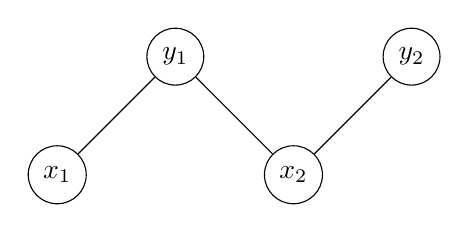
\begin{tikzpicture}[scale=1.5]
            \node (x1) at (0,0) [draw, circle] {$x_1$};
            \node (x2) at (2,0) [draw, circle] {$x_2$};
            \node (y1) at (1,1) [draw, circle] {$y_1$};
            \node (y2) at (3,1) [draw, circle] {$y_2$};
    
            \draw (x1) -- (y1);
            \draw (y1) -- (x2);
            \draw (x2) -- (y2);
        \end{tikzpicture}
    \end{center}

    If  $ M=\{(y_1,x_2)\} $, then the coverage expansion can only be  $ \{(x_1,y_1),(x_2,y_2)\} $ which does not intersect with  $ M $.  

    (c)
    It suffices to prove the network in (a) and the network in the lecture to find maximum matching returns the same value of min-cut.

    For any min-cut  $ (A,B)  $, since the edges from  $ X  $ to  $ Y  $ have capacity  $ \infty $, there is no edges from  $ A $ to  $ B  $ that belongs to the origninal biparite graph. So  $ c(A,B) $ in  $ (a) $ only calculates two parts: capacity from the source  $ s $ to  $ X\cap B $  and the capacity in  $ Y  $ side.
    
    Since  $ t\in B $, whether the middle nodes  $ n_y $ belongs to 
     $ A $ or  $ B $, it only calculates the capacity $ 1 $  from  $ y\in A  $ to  $ n_y $ once.
    And if  $ n\in A $, then capacity $ k $ from  $ n  $ to  $ t $ is calculated. Because the corresponding max-flow implies there is no edges from  $ y $ uncovered by  $ M' $ to  $ n $ cross  $ A $ and  $ B $, so  $ k=|A\cap\{y\text{ uncovered by  $ M' $}\}| $.     And if  $ n\in B $, it will calculates all capacity  $ 1 $  from  $ A\cap\{y\text{ uncovered by  $ M' $}\} $ to  $ n $ once.

    In short,  $ c(A,B)=|X\cap B|+|Y\cap A| $ for any  $ k $.
    
    However, to find maximum matching, the min-cut capacity is also  $ |X\cap B|+|Y\cap A| $.
    
    Then the size of maximum matching is $ K_2 $  $ \Rightarrow  $ $ \exists (A,B) $,  $ |X\cap B|+|Y\cap A|=K_2 $ $ \Rightarrow  $  $ k=K_2-|M'| $ is feasible for coverage expansion  $ \Rightarrow  $  $ K_1 \geq k+|M'| \geq K_2 $. 
    
    So  $ |K_1|=|K_2| $ 
    
    
    % It suffices to prove there is no matching whose size is  $ K_1+1 $.
    
    % WLOG, we assume nodes covered by  $ M $ is  $ y_1,y_2,\cdots,y_{K_1} $.
    % Then  $ \forall (x_i,y_j) $ edge in  $ G $,  $ j \geq K_1+1 $, since there is no larger coverage expansion of $ M'  $, for all matching  $ \{(x_{i_j},y_j)\}_{1 \leq j \leq K_1} $,  $ x_i\in \{x_{i_j}\}_{1 \leq j \leq K_1} $.
    
    % Now if there is some matching whose size is  $ K_1+1 $, WLOG we assume the matching is 
    % \[\{(x_{i_j},y_j)\}_{1 \leq j \leq t}\cup\{(x_{i_j},y_j)\}_{K_1+1 \leq j \leq K_1+K_1+1-t}\] 

    % Choose an arbitrary matching covering $ y_1,y_2,\cdots,y_{K_1} $ 
    % \[\{(x_{i_j}',y_j)\}_{1 \leq j \leq K_1}\]
    % Then  $ \{x_{i_j}\}_{K_1+1 \leq j \leq 2K_1+1-t}\subset \{x_{i_j}'\}_{1 \leq j \leq K_1} $, which means each  $ x_{i_j} $ has a corresponging connected $ y^j\in \{y_1,y_2,\cdots,y_{K_1}\} $.  However,  $ K_1+1-t \geq K_1-t $ implies that  $ \exists K_1+1 \leq j \leq 2K_1+1-t $,  $ y_{i_j} $ belongs to  $ \{x_{i_j}\}_{1 \geq j \leq t} $, WLOG, we assume  $ y^{K_1+1}=y_1 $, \ie  $ x_{K_1+1} $ is connected with  $ y_1 $.
    
    % Then for the sub-graph  $ (X,\{y_1,y_2,\cdots,y_{K_1},y_{K_1+1}\}) $, each  $ S\subset\{y_1,\cdots,y_{K_1}\} $ satisfies  $ |\Gamma(S)| \geq |S| $, where  $ \Gamma(S) $ is the nodes connected with  $ S $. And for each  $ S\subset\{y_1,\cdots,y_{K_1+1}\} $,   $ y_{K_1+1}\in S $,    
\end{problem}

\begin{problem}
    We can obtain a directed graph  $ G  $ in polynomial time that describes the nesting relation ship between each pair of boxes. Now suffices to find a minimum number of disjoint paths in  $ G $ that covers all nodes in  $ G $. 

    Now we use it to construct a network.

    First, there is a source node  $ s $, pointing to all boxes  $ i_{in} $, and a sink node  $ t $, pointed by all boxes $ i_{out} $, with capacity  $ \infty $. Here  $ i_{in}, i_{out} $ have the same meaning for the boxes but refers to different nodes. \ie There are two nodes representing the same box.

    If there is a directed edge  $ a\rightarrow b $ in  $ G  $, which means that  $ b $ is nest inside  $ a $, then we add an edge from  $ a_{in} $ to the node $ (a\rightarrow b) $ and an edge from the node $ (a\rightarrow b) $ to  $ b_{out} $. The capacity of these edges is  $ 1 $.
    
    We say an edge in  $ G $ is \textit{chosen} if the corrosponding connected edge in the network is saturated. 

    For this network, a feasible flow with integer value should satisfy:
    \begin{enumerate}
        \item edges in  $ G $ like  $ a\rightarrow x $ for  $ x $ unknown will be chosen once since the capacity to  $ a_{in} $ is  $ 1 $.
        \item edges in  $ G $ like  $ x\rightarrow b $ for  $ x $ unknown will be chosen once since the capacity from  $ b $ is  $ 1 $.
    \end{enumerate}

    So each nodes in  $ G $ connects with the input edge and the output edge that is chosen once.
    
    Therefore, the chosen edges in  $ G  $ forms several disjoint paths and some discrete nodes.


    Note that, the value of flow will be  $ \dps\sum_{(a\rightarrow b)\in G}f(a_{in}\to (a\to b)) $ which is the number of the chosen edges, denoted as  $ V $. Since several disjoint paths and some discrete nodes are actrually a forest,  $ V  $ also equals to  $ n- $the number of trees in the forest. So the number of trees in the forest is  $ n-V $, which implies that to minimize the number of trees in the forest, we actuall are to maximize the value of flow.

    So algorithm will be like this:

    \begin{enumerate}
        \item Construct a directed graph  $ G  $ in polynomial time that describes the nesting relation ship between each pair of boxes.
        \item Construct a network with  $ G  $ as we discussed above.
        \item Use the Capacity-Scaling Algorithm to find a maximum flow in the network.
        \item The number of disjoint paths is  $ n-V $, where  $ V $ is the value of flow.
    \end{enumerate}
     $ n-V $ is what we need.

    The running time complexity is just the same as the time complexity of algorithm to find a single max-flow with at most $ 2+2n+\frac{n(n-1)}{2} $ nodes and  $ n(n-1)+2n $ edges, which is  $ O(n^5) $. 

\end{problem}



\end{document}